\documentclass[bachelor,zhspacing]{cqu}  %单面打印版本
\usepackage{etex}
\def\tightlist{}

%%在这增加你需要的其它包
\definecolor{hellgelb}{rgb}{1,1,0.8}
\definecolor{colKeys}{rgb}{0,0,1}
\definecolor{colIdentifier}{rgb}{0,0,0}
\definecolor{colComments}{rgb}{1,0,0}
\definecolor{colString}{rgb}{0,0.5,0}
\usepackage{listings}
\lstset{%
    float=hbp,%
    basicstyle=\ttfamily\small, %
    identifierstyle=\color{colIdentifier}, %
    keywordstyle=\color{colKeys}, %
    stringstyle=\color{colString}, %
    commentstyle=\color{colComments}, %
    columns=flexible, %
    tabsize=4, %
    frame=single, %
    extendedchars=true, %
    showspaces=false, %
    showstringspaces=false, %
    numbers=left, %
    numberstyle=\tiny, %
    breaklines=true, %
   backgroundcolor=\color{hellgelb}, %
    breakautoindent=true, %
    captionpos=b,%
	xleftmargin=0pt%
}

\begin{document}

%-----------------------------------论文题目-------------------------------------------------
\xuehao{20121892}
\cntitle{基于深度学习的自增长图片验证码系统}
\cnauthor{张乐}
\cnmajor{软件工程}
\cnteacher{葛永新}
\cnxueyuan{软件学院}
\entitle{Automatic Increased Image-based CPATCHA with Deep Learning}
\enauthor{Le Zhang}
\enmajor{Software Engineering}
\enteacher{Prof. Yongxin Ge}
\enxueyuan{College of Software}
\cnkind{****}
\enkind{****}
%\cnzlteacher{ }  %%助理教师,如果必要,还要将cqu.cls中的有关该项前的%号去掉
%\enzlteacher{ }
\cndate{二O一六年六月}
\endate{June 2016}
%%%%只需修改上面的相关信息%%%%%%%%
\makecntitle 
\makeentitle 
%%%%%%%%%%%%%%%%%%%%%%%%%%%

\pagenumbering{Roman}
\setcounter{page}{0}
%------------------------------------文章摘要------------------------------------------------------------
\cnkeywords{深度学习,自增长,图片验证码,爬虫,大数据}
\begin{cnabstract}
摘要是设计或论文内容不加注释和评论的简短陈述,应以第三人称陈述。它应具有独立性和自含性,
即不阅读设计或论文的全文,就能获得必要的信息,摘要的内容应包含与设计或论文同等量的主要信
息,供读者确定有无必要阅读全文,也供文摘等二次文献采用。\par
摘要一般应说明研究工作目的、实验研究方法、结果和最终结论等,而重点是结果和结论。摘要中一
般不用图、表、化学结构式、计算机程序,不用非公知公用的符号、术语和非法定的计量单位。\par
摘要页置于英文题名页后。 \par
中文摘要一般为400汉字左右,用小四号宋体。 \par
关键词是为了文献标引工作从设计(论文)中选取出来用以表示全文主题内容信息款目的单词或术
语。一般每篇设计(论文)应选取3~5个词作为关键词,关键词间用逗号隔开,最后一个词后不打标点
符号。以显著的字符排在同种语言摘要的下方。如有可能,尽量用《汉语主题词表》等词表提供的规
范词。\par
本文介绍重庆大学论文模板cqu的使用方法。本模板符合学校的本科论文格式基本要求,而硕博模板
有待完善。
本文的创新点主要有:
\begin{itemize*}
\item 用例子来解释模板的使用方法;
\item 用废话来填充无关紧要的部分;
\item 一边学习摸索一边编写新代码。
\end{itemize*}
\end{cnabstract} 

\enkeywords{Deep Learning, Automatic Increase, Image-based CPATCHA, Crawler, Big Data}
\begin{enabstract}
     An abstract of a dissertation is a summary and extraction of 
research work and contributions. Included in an abstract should be 
description of research topic and research objective, brief 
introduction to methodology and research process, and summarization 
of conclusion and contributions of the research. An abstract should be 
characterized by independence and clarity and carry identical 
information with the dissertation. It should be such that the general 
idea and major contributions of the dissertation are conveyed
without reading the dissertation.\par
     An abstract should be concise and to the point. It is a 
misunderstanding to make an abstract an outline of the dissertation and 
words “the first chapter”, “the second chapter” and the like should be 
avoided in the abstract.\par
     Key words are terms used in a dissertation for indexing, 
reflecting core information of the dissertation. An abstract may 
contain a maximum of 5 key words, with semicolons used in between to 
separate one another.
\end{enabstract}
%%%%%%%%%%%%%%%%%%%%%%%%%%%%%%%%%%%%%%

%--------------文章目录-------------
\tableofcontents
\listoffigures
%\addcontentsline{toc}{section}{插图清单}
\listoftables
%\addcontentsline{toc}{section}{附表清单}


%------------------------------------词汇------------------------------------------------------------
\begin{denotation}{2.5}{0}


\item[问题] 验证码系统通过向用户提问来区分人和机器,本文中特指验证码系统提问内容。
\item[主体] 一张图片中可能包含多个物体,本文中将图片中的单个物体称为主体。

\item[Q] 某次生成\emph{问题}的图片集合。

\item[Qu] 生成问题中非确信\emph{主体}集合。
\item[Qc] 生成问题中起验证作用的确信\emph{主体}集合。

\item[I] 数据库中所有\emph{主体}的集合。
\item[Iu] 是一个集合,表示非确信\emph{主体}集。
\item[Ic] 是一个集合,表示确信\emph{主体}集。

\item[N] 数据库中所有\emph{主体}名称的集合。
\item[Nu] 是一个集合,数据库中所有非确信\emph{主体}名称的集合
\item[Nc] 是一个集合,数据库中所有确信\emph{主体}名称的集合


\end{denotation}

%%%%%%%%%%%%%%%%%%%%%%%%%%%%%%%%%%%%%%%

\pagenumbering{arabic}

\section{前言}\label{ux524dux8a00}

当今人们越来越依赖Web服务,如查看E-mail,淘宝购物,百度搜索,这些Web服务已经和我们息息相关,我们很难想象没有他们的生活。而对于这些服务的提供者来说,确保服务资源能真正被用户使用,而不是被恶意机器人使用,是至关重要的。如使用机器人注册账户\textsuperscript{{[}1{]}},不仅会占用宝贵服务器资源,还为发布恶意信息埋下伏笔。所以区分访问来自人类还是机器人是十分重要的,验证码正是因为这个原因而被广泛使用。验证码(CAPTCHA)是``Completely
Automated Public Tests to tell Computers and Humans
Apart''\textsuperscript{{[}1--5{]}}。的缩写。其主要思想是通过电脑向人类提问,通过回答来区分人和机器人。这个问题需要对人来说简单,而对电脑来说很难(或是需要很长时间)解决。常见的验证码系统主要分为三类:文本验证码系统,声音验证码系统,图片验证码系统。文本验证码系统容易被破解{[}{[}6{]};{[}7{]};el2010robustness{]},且对移动用户不友好;声音验证码系统由于设备限制,相比于文本验证码系统并没有显著提高安全性等原因,并没有被广泛的使用;而图片验证码系统,因为其安全性以及良好的用户体验,被越来越多的使用。然而验证码系统也存在一些问题:a)需要人工建立图片库;b)人工建立的图片库质量无法保证;c)图片来源单一。正是普通的图片验证码系统纯在这样的问题,为解决这些问题,本文提出了一种基于深度学习的自增长图片验证码系统。

\section{背景}\label{ux80ccux666f}

目前在互联网上最流行的CAPTCHA系统,是基于文本的。但是,由于计算机视觉技术的提高,基于文本的系统很容易被攻击成功\textsuperscript{{[}6--8{]}}。所以越来越多的研究者考虑如何替换掉基于文本的系统,于是有基于图像的\textsuperscript{{[}9--14{]}}和基于声音的\textsuperscript{{[}15,16{]}}系统。

\subsection{文本验证码系统}\label{ux6587ux672cux9a8cux8bc1ux7801ux7cfbux7edf}

总的来说,基于文本的验证码系统让用户识别字母或数字,GIMPY是一个经典的例子\textsuperscript{{[}17{]}}。攻击基于文本的使用大多使用OCR(optical
character
recognition)。这个技术讲图片分割成晓得区域,每个区域只有一个字母,然后使用模式识别技术使用字母模板匹配每一个区块\textsuperscript{{[}6--8{]}}。最后一步是一个比较成熟的AI问题。为了防止这样的攻击,基于文本的系统使用如下技术来增强鲁棒性\textsuperscript{{[}2,18{]}}:

\begin{itemize}
\tightlist
\item
  增加噪音:向图片中增加线和点,来干扰区域分割算法。
\item
  字符扭曲:对字符使用扭曲变换,或3D变换来增加文字识别难度。
\item
  字符连接或重叠:将两个或者多个字母连接或者重叠起来,使得攻击算法无法正确划分图片。
\end{itemize}

\begin{figure}[htbp]
\centering
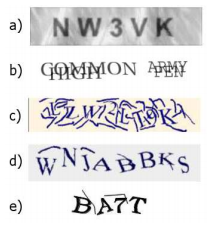
\includegraphics{pic/text-captcha.png}
\caption{一些文本CAPTCHA的例子}\label{fig:text-captcha}
\end{figure}

如 图~\ref{fig:text-captcha}
,a)很容易被OCR破解,b)引入了字符的重叠,c)引入了噪声,d)和e)同时引入噪声和字符扭曲。

然而,以上方法在提高系统鲁棒性的同时,也提高了人类识别的难度,特别是字符的连接。如字符``r''和``n''连接起来,看起来就像是字符``m''。字符扭曲也有可能增加用户识别的难度,如扭曲的后的''S``和''5``就很难分辨。还有些系统使用不同的颜色来标示每个字符,而这些都能很容易的被自动化的程序所移除,并没有给机器识别带来任何的难度\textsuperscript{{[}19{]}}。而reCAPTCHA\textsuperscript{{[}20{]}}提供了一种比较好的解决思路:使用两个单词来验证用户。其中一个是确定答案的,另外一个是不确定的。不确定答案的单词来自古籍中无法被自动化OCR程序识别的单词,确定答案的单词是机器生成的或者多个用户的答案是一致的来自古籍中的单词。这个过程既可以起到验证作用又可以数字化图书,是一个非常好的解决方案。但是还是这个解决方案还是有如下缺点:

\begin{itemize}
\tightlist
\item
  对移动用户不友好:移动设备通常屏幕较小,输入困难,输入较长的单词对用户来说是一个极大的负担。
\item
  无法防御基于机器学习的攻击:基于机器学习的攻击,能比较容易的识别文本,此方法对与基于机器学习的攻击没有很好的鲁棒性。
\item
  易导致用户多次刷新:由于一个单词来自古籍,可能出现用户多次刷新来获得清晰可读的验证码,而这对热门Web服务器来说,是一个极大的负担。
\end{itemize}

正是由于基于文本的系统固有的缺点,有了声音验证系统和图像验证码系统。

\subsection{声音验证码系统}\label{ux58f0ux97f3ux9a8cux8bc1ux7801ux7cfbux7edf}

声音验证码系统弥补来了视觉障碍用户的可用性需求。一般的声音验证码系统用随机的声音间隔将字母和数字被隔开,并向声音中添加背景噪声。用户只有很少的时间去确定每个单词。某种意义上说,声音验证码系统仅仅是文本验证码系统的听觉版本,用声音替代可视化的东西,并没有明显的增加破解的难度。构成攻击的基础是相似的------特征提取和字符分类。对机器和人的难度曲线是相似的\textsuperscript{{[}21{]}}。所以声音验证码系统既没有提供更加用户友好的接口,也没有更好的防范自动化程序的破解。这也就是它没有被广泛使用的根本原因。

\subsection{图像验证码系统}\label{ux56feux50cfux9a8cux8bc1ux7801ux7cfbux7edf}

图像验证码系统逐渐替代了越来越复杂的文本验证码系统,图像验证码有很好的用户接口,它主要利用人类对图片超乎想象的处理能力来区分人和机器。ESP-PIX\textsuperscript{{[}22{]}}让用户从一系列词中选择能描述素有图片的。SQ-PIX\textsuperscript{{[}23{]}}让用户标示出物品的所在位置,这对图片候选库提出很大要求,大部分图片可能需要人工处理。Google的图片验证码``what's
up''\textsuperscript{{[}10{]}}让用户把图片旋转至正确方向。这个过程需要比较精确的鼠标移动,并且有些图片的方向可能是模棱两可的。Microsoft的Asirra\textsuperscript{{[}9{]}}使用petfinder.com上已有的数据库,让用户在12张图片中找到所有有猫的图片(其他图片都为狗)。而这些图片可能是模棱两可的,如
图~\ref{fig:asirral}
中,左图中既有猫也有狗,右图中有一只长得像狗一样的猫。这样的验证码这个对于机器来说,难度只有区分狗和猫,而对于人来说,却可能花费很长时间解决。

\begin{figure}[htbp]
\centering
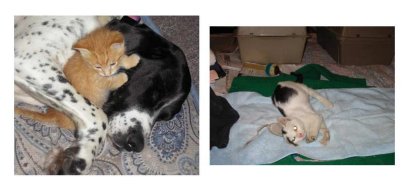
\includegraphics{pic/asirral.png}
\caption{petfinder.com中模棱两可的图片}\label{fig:asirral}
\end{figure}

12306火车购票\textsuperscript{{[}24{]}}让用户从所有图片中选择系统指定内容的图片,如
图~\ref{fig:12306captcha}
。但是同样也存在一个致命的问题:图片需要人工导入,并手动指定标签。有如下缺点:

\begin{itemize}
\tightlist
\item
  人工失误:人工指定标签时给出错误标签
\item
  易遭受穷举攻击:因为人工指定,图片库不可能太大,穷举所有图片,并自动或手动指定标签即可很好的破解此类验证码
\item
  手工录入的标签信息很难复用:花费大量人力物力输入的信息除了验证码,并不能用在其他地方。
\end{itemize}

\begin{figure}[htbp]
\centering
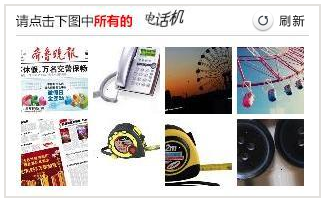
\includegraphics{pic/12306captcha.png}
\caption{12306验证码}\label{fig:12306captcha}
\end{figure}

正是由于图片验证码系统普遍有需要手动录入图片的缺点,本文提出了一种\textbf{图片数据库自增长}的方案来解决这个问题。

\section{图片验证码自增长系统设计}\label{ux56feux7247ux9a8cux8bc1ux7801ux81eaux589eux957fux7cfbux7edfux8bbeux8ba1}

不同于文本验证码系统,文本验证码系统可以生成问题图片,而图片验证码系统生成问题的过程很依赖图片数据库。这就决定图片数据库是图片验证码系统中至关重要的角色。图片数据库的的数据量大小和质量好坏,直接影响图片验证码系统的鲁棒性和用户友好性。数据量大能很好的避免穷举攻击,而数据质量高,能很好提升系统的用户友好性。如何提高图片数据库的数据量和数据质量,成了现在大多数验证码系统亟待解决的问题\textsuperscript{{[}11{]}}。本文创新性的提出了一种图片验证码系统图片数据库自增长策略,能很好的解决这个问题。同时,本系统在设计之初就考虑到图片数据库复用问题:利用海量数据,服务于图片语义化搜索。这使得本系统合理利用用户完成验证码过程中输入,为搜索引擎的图片语义化搜索做出贡献。

\subsection{思路}\label{ux601dux8def}

reCAPTCHA系统是基于文本的验证码系统,是借助于人类大脑对难以识别的字符的辨别能力,进行对古旧书籍中难以被OCR识别的字符进行辨别的技术。这是一个很好的''增长``思路。本系统参考了reCAPTCHA系统,将其改进以适应图片验证码系统。

\subsubsection{reCAPTCHA系统}\label{recaptchaux7cfbux7edf}

每次验证码会显示两个单词让人来识别,其中一个是需要用户识别的难认词,另外一个是答案已知的词。软件将能够正确识别答案已知词的用户看作是人类,当答案已知的词被正确识别出来后,程序会记录用户对无法阅读的词的回答并将其添加到它的数据库中。这样就完成了一次人工的OCR识别。为了改善软件的精确性,
reCAPTCHA
会将最困难的词发送给多个用户并挑选其中有相同答案的作为正确的答案,确率能够达到99\%。用户每使用一次这个程序,实际上就是在帮助数字重现古籍。这项技术已经被Google广泛使用。

reCAPTCHA系统提供了很好的利用用户输入来完成某种目的的思路。即利用用户对OCR无法识别单词的输入,完成古籍数字化工作。相思的思想可以用在图片验证码系统上吗?答案是肯定的。我们可以让\textbf{用户选择两种物体,其中一个的答案是确定的,起验证作用;另外答案一个是不确定的,起系统自增长作用}。但是在实施的时候,任然需要对reCAPTCHA系统进行很多改进,才能使之很好的用在图片验证码系统上。

\subsubsection{图片验证码的自学习与reCAPTCHA系统差异}\label{ux56feux7247ux9a8cux8bc1ux7801ux7684ux81eaux5b66ux4e60ux4e0erecaptchaux7cfbux7edfux5deeux5f02}

图片验证码的自学习策略并不能直接把reCAPTCHA系统思路方案拿来使用,这由于图片验证码系统和文本验证码系统有着本质的区别:

\begin{itemize}
\tightlist
\item
  验证问题生成:图片验证码依赖图像数据库,而reCAPTCHA系统一般是由系统随机选择一个单词,然后由系统生成一张包含单词图片交由用户识别。
\item
  用户输入类型:图片验证码一般是让用户点击选择图片,而reCAPTCHA系统是让用户输入图片中的文本。
\item
  图像分割:图片验证码需要预先将一张图片上物体分离出来,而reCAPTCHA系统只需要讲古籍上的单个字体提取出来,这个二者的难度完全不在一个量级。
\item
  预识别:图片验证码需要预先对图片加上描述标签,而reCAPTCHA系统并不需要任何预识别。
\end{itemize}

正是由于以上差异,图片验证码系统自学习系统要比reCAPTCHA复杂得多。其中特别是图像分割\textsuperscript{{[}25--28{]}}和预识别\textsuperscript{{[}29--31{]}}部分,涉及计算机视觉以及人工智能领域。

\subsubsection{自增长策略}\label{ux81eaux589eux957fux7b56ux7565}

不同与reCPATHCHA,我们可以讲古籍中的单词抠出后,经过少许处理即可交由用户。图片自学习系统不太可能设计成让用户输入图片中物体的名称,因为多个用户输入的图片名称可能是多个近义词或同义词的集合,如:土豆和马铃薯,这样就没有办法很好的规约图片中主体的名称。正是考虑到这个因素,我们需要对图片进行预识别,然后通过用户选择图片这一过程来验证机器的识别。即:需要用户选择带有两种标签的全部图片,其中带有确信标签(确信标签为
\texttt{true})图片起到真正的验证作用,而用户是否选择非确信标签(确信标签为
\texttt{false})的图片作为验证机器识别的依据。

大体过程如下:

\begin{enumerate}
\def\labelenumi{\arabic{enumi}.}
\tightlist
\item
  将 \href{http://groups.csail.mit.edu/vision/TinyImages/}{Visual
  Dictionary} 中带有标签图片的数据输入数据库中,并将他们的确信标签置为
  \texttt{true}
\item
  使用预先有标签的图片数据集训练深度神经网络,使其具备初级的图片识别能力
\item
  通过爬虫从网络上爬取图片
\item
  将爬取图片筛选,初步处理
\item
  将图片分割(image segmentation)成带有物体的子图(也就是\emph{主体})
\item
  使用具有初级图片识别能力的深度神经网络对图片标定预标签(标定多个标签,按置信度排序)
\item
  将识别结果存入图片数据库中,并置确信标签为 \texttt{false}
\item
  按一定比例使用确信标签为 \texttt{true} 和 \texttt{false}
  的\emph{主体}生成图片验证码\emph{问题}
\item
  将用户验证成功的\emph{问题}中是否选中确信标签为 \texttt{false}
  的\emph{主体}信息记录到数据库中
\item
  当确信标签为 \texttt{fasle}
  的\emph{主体}验证次数和准确率都超过预先设定的阈值时,将确信标签置为
  \texttt{true};当确信标签为 \texttt{fasle}
  的\emph{主体}验证码次数超过,而准确率低于预先设定的阈值时,将标签置换为下一标签(置信度仅此与当前标签的标签),重置验证次数和准确率
\item
  按一定时间时间或者按由 \texttt{false} 转为 \texttt{true}
  的标签数量达到预先设定的值时,使用\emph{主体}继续训练深度神经网络
\end{enumerate}

顶级流程图如 图~\ref{fig:flow}。

\begin{figure}[htbp]
\centering

\includegraphics{pic/cqu.eps}
\caption{自增长的图片验证码系统顶级流程图}\label{fig:flow}
\end{figure}

\subsection{设计}\label{ux8bbeux8ba1}

本系统希望达到如下目标:

\begin{itemize}
\tightlist
\item
  适应人类:自动淘汰图片数据库中含糊不清的图片,去掉模棱两可的图片,更加逼近人类去图片的理解
\item
  自动增长:通过爬虫自动下载网络上的图片,自动将图片分割成\emph{主体}并预识别图片中的内容,打上预识别标签。
\item
  合理验证码生成:通过使用合理比例确信与不确信的主体来生成验证码,使得:1)
  可以验证访问是否是人类;2) 能为系统自增长提供依据
\item
  Web服务:实现自增长,需要数以亿记的用户使用长期使用才能达到自增长目的。所以我们期望将系统设计为Web服务类型,向其他网站提供服务,来提高自己的用户量。这其中需要解决两个问题:1)
  大并发访问;2) 服务认证
\end{itemize}

正是基于上面的考量,本系统在设计时需考虑多个因素,使得本系统,人性化,用户友好,并有很好的鲁棒性。

\subsubsection{手动输入}\label{ux624bux52a8ux8f93ux5165}

在系统未形成规模前,需要手动向数据库中导入一些图片,所以系统需要为手动输入提供接口。最好还需要提供图片裁剪接口,如
图~\ref{fig:manual-ui}

\begin{figure}[htbp]
\centering
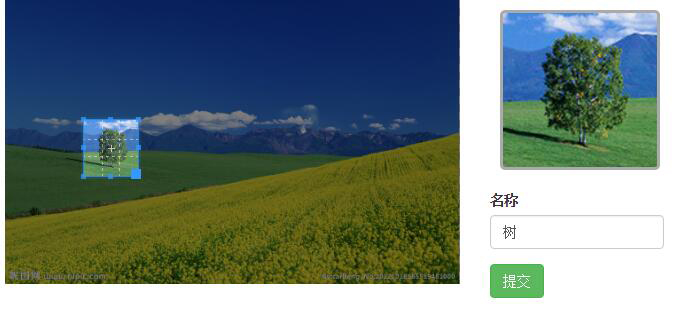
\includegraphics{pic/manual-ui.jpg}
\caption{手动输入UI}\label{fig:manual-ui}
\end{figure}

\subsubsection{适应人类}\label{ux9002ux5e94ux4ebaux7c7b}

本系统的初始确信图片为
\href{http://groups.csail.mit.edu/vision/TinyImages/}{Visual Dictionary}
中带标签的图片数据,然而这些图片中可能存在模棱两可或是模糊不清的图片。如果使用这样的图片来判定用户是否为人类,可能造成:

\begin{itemize}
\tightlist
\item
  判定失误:有些图片对人类来说也是很难辨认的
\item
  丧失用户友好性:用户可能对验证过程厌恶
\item
  高服务器负载:本系统设计为 Web
  服务,本身存在高并发问题。如果使用这样的图片,会大大提高用户刷新验证码的概率,进而提高服务器负载
\end{itemize}

可见,数据库中如果存在模棱两可或是模糊不清的图片可能会对系统造成毁灭性打击,所以如何降低这种图片在数据库中的比例尤为重要。

我们的系统引进了一种\textbf{淘汰机制}。具体实现如下:

\begin{enumerate}
\def\labelenumi{\arabic{enumi}.}
\item
  记录所有\emph{主体}总共出现次数和答对概率
\item
  设计定时任务计算所有出现次数大于阈值的\emph{主体}答对概率的均值
  \(\mu\) 和 \(\sigma\)
\item
  淘汰所有答对概率低于 \(\mu-3\sigma\) 的\emph{主体}
\end{enumerate}

这里我们根据概率统计中的大数定理可知,任意分布的样本,在取样足够大时,无线逼近正态分布。在这里使用
\(3\sigma\) 原则,可以在理论上保证正确排除异常样本。

\subsubsection{图片爬虫}\label{ux56feux7247ux722cux866b}

为实现自增长,系统系统需要不断的从互联网上爬取图片来实现系统数据库的自增长。为了这个目的,我们需要使用爬虫来爬取互联网上图片。相比与其他复杂爬虫,这里的爬虫相对简单:只需要下载互联网上图片即可。

\paragraph{爬虫策略}\label{ux722cux866bux7b56ux7565}

爬虫是一种定向抓取网页资源的程序,它根据抓取目标,有选择的访问互联网上的网页与相关连接来获取所需要的信息。在我们的系统中,爬虫的任务很简单:下载互联网上的图片。

目前主流的爬虫网页搜索策略为以下3种:

\begin{itemize}
\item
  广度优先搜索:广度优先搜索策略是类似于图遍历算法中的广度优先算法,即指搜索过程中,当完成当前节点邻接节点搜索后,才进行邻接节点的邻接节点搜索。目前为了尽可能多的涵盖所有网页,一般使用这种方法。其基本思想是很大概率上与初始链接在一定距离内的网页具有主题相关性。一般配合网页过滤技术,将无关网页过滤掉。缺点是抓取网页增多,会将大量无关网页下载并过滤掉,让其执行效率变低。
\item
  最佳优先搜索:最佳搜索是按一定的算法,预测候选链接与目标网页的相似度,或主体相关性,将其从大到小排列,选取前几个来你就进行搜索。这种算法某种意义来说,是一种贪婪算法,容易陷入局部最优解而不能很好的获得结果。因此需要将最佳优先搜索策略结合具体应用场景进行改进,来跳出局部最优点。
\item
  深度优先搜索:深度优先搜索策略从起始网页开始,选择一个链接进入,分析这个网页中的链接,选择一个再进入。如此抓取下去,直到一条路线处理完成之后再处理下一条路线。该算法的设计和实现相对简单。这种策略抓取深度直接影响着抓取命中率以及抓取效率,抓取深度的合理设定是该种策略的关键。相对来说,这种策略很少使用。
\end{itemize}

我们系统中需要抓取包含尽可能多的\emph{主体}的图片(准确来说是单位像素包含主体最多的图片,我们的系统要求\emph{主体}不能过小,以至于模糊不清)。需要做到:

\begin{itemize}
\item
  固定搜索域:我们的期望下载的图片是包含多个主体的,而互联网上的图片很难保证这点,所以我们需要固定搜域到某个网站下,以免爬虫跳出。具体选择那个网站作为我们图片的来源,这里涉及版权、法律和政治问题,需要考虑很多因素,这里不再详细说明。
\item
  筛选图片:对网站背景之类的图片予以过滤,并过滤掉较小的图片。
\item
  保证相关性:可以认为相关的图片内容项可能是相似的,我们要求图片中尽可能多的包含\emph{主体},这就要求我们的找到的图片,和拥有多的\emph{主体}的图片是相关的。
\item
  剔除重复:爬虫需要多次上次爬图片,爬到的图片可能是之前已经爬到的,这就需要我们的爬虫具备自动剔除重复图片的能力。
\end{itemize}

综上,最佳搜索策略是最适合的选择。其最佳评价取决于图片主题的关键字;即假定:主体相思的图片是相似的。

\subsubsection{图片分割}\label{ux56feux7247ux5206ux5272}

从网上爬取的图片一般来说,内容杂乱,主体不明,我们期望的拉去图片如
图~\ref{fig:download-image} 中的
a),然而实际拉取的图片可能存在以下问题:

\begin{enumerate}
\def\labelenumi{\arabic{enumi}.}
\item
  一张图片包含多个\emph{主体}:大多数的图片是包含多个\emph{主体}的,主体之间可能是重叠的,互相遮蔽的。如
  图~\ref{fig:download-image} 中的 b)。
\item
  图片可能不包含\emph{主体}:有些图片,如桌面壁纸类的图片可能不包含任何\emph{主体},如
  图~\ref{fig:download-image} 中的 c)。
\end{enumerate}

正是存在这些问题,我们非常有必要对图片进行分割:对于包含多个\emph{主体}的图片,分割出\emph{主体}子图:对于不包含\emph{主体}的图片,理想分割出0个\emph{主体}子图。

\begin{figure}[htbp]
\centering

\includegraphics{pic/cqu.eps}
\caption{爬虫拉取的部分图片}\label{fig:download-image}
\end{figure}

图像分割是一个比较难解决的问题,常见分割算法有:

\begin{itemize}
\item
  基于阈值的分割方法:阈值分割直接对图像灰度信息阈值化处理,它简单的使用几个阈值在图像灰度直方图上分类,将灰度值在同一个类内的像素归为同一个物体
  {[}27{]}
  。其实现简单、成本低廉、实用性强;但当图像灰度不明显,或是多个物体灰度有较大重叠时,容易分割错误
  {[}27{]} 。
\item
  基于边缘的分割方法:图像中突变的出现一般伴随着边缘的出现,换句话说是不同\emph{主体}之间像素灰度值变化往往比较剧烈;根据高等数学的有关知识:可知图片的一阶导数和二阶导数往往反应了图片中突变信息,因此这类方法一般采用图片一阶导数和二阶导数满足某种约束作为边缘点的判断依据,其优点:准确性高,效率高;其局限性:边缘连续性和封闭性难以保证,对于复杂图像分割效果差,会出现如:边缘模糊、边缘丢失等现象。边缘检测方法常常依赖于边缘检测算子,常用的检测算子有:Sobel(对噪声具有一定平滑,但精度低)、Roberts(精度高、对噪声敏感)、Canny(检测阶跃型边缘效果好,抗噪强)、Prewitt、Laplacian和Marr。
\item
  基于区域的分割方法:这类方法主要考虑了图像的空间信息,如图像纹理、颜色、灰度和像素的统计特性等,进而将目标对象划分为同一区域的分割方法。常见的区域分割方法主要有:区域生长法、分水岭分割法和分裂合并法。
\item
  基于小波的图像分割方法:小波(Wavelets)是目前在许多工程和科学技术中一个非常热门的话题。它具有良好的视频局部变化和多尺度变换特性,以及多分辨率分析的能力
  {[}32{]}
  。在二维空间情况下,信号的突变点对应于小波变换模的极大值点;小波变换可以检测
  图像的空间局部奇异性,故可确定图像的边缘。
\item
  基于人工神经网络的图像分割方法:人工神经网络(ANN)是大规模神经元互联组成的高度非线性系统,是在认识、理解人脑的组织结构和运行机制的基础上,模拟其结构和智能行为的一种工程系统。基于神经网络图像分割方法的基本思想是:通过训练多层感知器(Perceptron)来得到决策函数,然后用决策函数对象素进行分类来达到分割目的。
\end{itemize}

TODO:

\subsubsection{图像预识别}\label{ux56feux50cfux9884ux8bc6ux522b}

TODO:

\subsubsection{验证码生成}\label{ux9a8cux8bc1ux7801ux751fux6210}

验证码生成策略是整个系统最为关键的一步,本系统生成的验证码需要实现:a)区分人和机器;b)收集用户输入来实现系统自增长。因此需要合理的设计验证码生成策略。

这里以生成12306火车购票验证码\textsuperscript{{[}24{]}}为例,说明验证码生成策略。其他图片验证码系统如SEMAGE\textsuperscript{{[}33{]}}也可以采用相思的思想,在本策略上稍加修改,即可实现验证码系统自增长。为了方便的说明验证码生成策略,在这里引入一些符号(其他符号请参考主要符号对照表):

\begin{itemize}
\item
  \(Name(x)\):\(x\)为\emph{主体},\(Name(x)\)为主体当前所对应的名称(对确信或是非确信主体都成立)
\item
  \(Qcc\):\(Qc\)的子集,\emph{问题}题干中确信名称对应的全体\emph{主体}集合
\end{itemize}

为了使生成的验证码不混淆(即通过用户答案,并不能判断用户是否通过验证),验证码生成需要满足如下条件(注意:这里只是一个充分条件,其他能保证验证码不混淆的约束也是可行的):
\begin{equation}\forall x_i,x_j \in Qu , Name(x_i) = Name(x_j)\label{eq:Qu-consistency}\end{equation}
\begin{equation}\forall x_i,x_j \in Qc , Name(x_i) = Name(x_j)\label{eq:Qc-consistency}\end{equation}
\begin{equation}\forall x_i \in Qc-Qcc ,\forall x_j \in Qu \cup Qcc , Name(x_i) \neq Name(x_j)\label{eq:No-conflict}\end{equation}

公式~\ref{eq:Qu-consistency} 和 公式~\ref{eq:Qc-consistency}
分别表明\(Qu\)和\(Qc\)中的\emph{主体}名称应该相同;而
公式~\ref{eq:No-conflict}
表明用来``充数''的\emph{主体}名称应该与用来测试用户是否为人类和验证预识别结果所使用的\emph{主体}名称不同。这样即能保证生成的验证码是不混淆的。

\subsubsection{置信标签修改}\label{ux7f6eux4fe1ux6807ux7b7eux4feeux6539}

所谓置信标签修改即为当用户提交足够多次验证后,系统自动将某些\emph{主体}的置信标签修改掉。这一过程是系统自增长的最终表现方式,通过将置信标签为\texttt{false}的\emph{主体}修改为\texttt{ture}完成。在我们的系统里,采用阈值法完成修改触发:即图片出现次数大于某个值,并且用户先选择比例大于一定值时,将置信标签修改。

为了说明这个策略的合理性,我们不妨举如下例子:

假设我们的系统的图片预识别深度神经将某一\emph{主体}认为为``梨子'',假设生成的验证码\emph{问题}是``请选择所有的XX,梨子'',其中XX是确信的。那么如果有足够比例的用户选择了这个\emph{主体},那么我们就可以认为,这个\emph{主体}就是``梨子'',因为它通过了大部分的人类识别。

\subsubsection{Web 服务}\label{web-ux670dux52a1}

我们的自增长系统需要数以亿计的用户使用,才能实现良好的自增长。为此仅仅嵌入到几个网站中使用并不能达到我们的目的。所以
Web 服务是最好的选择,即提供一定的 API
给用户,用户调用即可完成``全自动区分计算机和人类的图灵测试''。这里称提供CAPTCHA服务的服务器为验证服务器,提供
Web 应用服务的服务器为应用服务器,用户为客户机。

\paragraph{基本模型}\label{ux57faux672cux6a21ux578b}

把验证过程做成服务,也就是别的平台(网站)在需要验证用户是否为人类时,通过将\emph{问题}与某次web请求(一般以提交表单形式)绑定,用户通过人类测试以后,应用服务器才处理那个请求,否则将忽略它。

\begin{figure}[htbp]
\centering

\includegraphics{pic/cqu.eps}
\caption{Web 服务交互图}\label{fig:base-interaction}
\end{figure}

如 图~\ref{fig:base-interaction}
,首先应用服务器向客户机提供表单唯一id。客户机填写表单完成提交之前,需要请求验证服务器,获取\emph{问题}和\emph{问题}的UUID。正确回答\emph{问题}后,将UUID连着表单一同提交给应用服务器。应用服务器根据客户机的提交的UUID访问验证服务器,获取当前UUID是否验证通过,是否只使用一次等信息,即可知道用户是否通过验证。

\paragraph{数字签名}\label{ux6570ux5b57ux7b7eux540d}

上面的方案虽然可以完成验证码过程,但是可以很清楚看到:验证服务器,应用服务器,客户机需要至少\(6\)次通信,才可以完成这一过程。经过仔细分析,我们发现可以通过数字签名方式,在保证原有功能和安全性的基础上,将通信次数降为\(4\)次。

\begin{figure}[htbp]
\centering

\includegraphics{pic/cqu.eps}
\caption{Web
服务交互图(数字签名版)}\label{fig:digital-signature-interaction}
\end{figure}

如 图~\ref{fig:digital-signature-interaction}
。首先应用服务器向客户机提供表单唯一id,客户机填写表单完成提交之前,请求验证服务器获取\emph{问题}时,需要将表单唯一id提交给验证服务器。客户机正确回答问题后,将获得由验证服务器私钥加密的表单唯一id(这里称密文)。而后客户机需要将这个密文连同表单一起发给应用服务器。应用服务器只需要用公钥解密,验证密文解密后的内容是否与表单唯一id一致,即可知道用户是否通过了验证。

由于数字签名方案,从验证服务器角度看,减少了\(\frac{1}{3}\)的请求。这对于访问密集型的应用来说,是一个极大的优化。也就是说,相同配置的服务器,可以多容纳\(\frac{1}{3}\)的请求。因此在大数据和海量并发的应用场景中,数字签名方案是最佳选择。

\section{图片验证码自增长系统分设计析}\label{ux56feux7247ux9a8cux8bc1ux7801ux81eaux589eux957fux7cfbux7edfux5206ux8bbeux8ba1ux6790}

\subsection{可用性}\label{ux53efux7528ux6027}

系统的可用性基本等同与其他类型的图片验证码:人类利用存储的常识,可以让用户花费很少的功夫来解决问题。同样由于图片验证码系统的先天优势:完成验证只需要点击输入,而不需要键盘输入,使得我们的验证码系统在触屏移动设备上表现良好。

我们的系统还存在一个自增长策略,即通过用户输入来增加图片数据库,其中图片预识别是一个很关键的步骤。\textbf{不难得出,图像识别深度神经网络的识别率并不影响系统的验证性能和增长数据质量,其影响的只是系统自增长速率}。我们系统里的深度神经网络可以不断利用系统自增长获得的``知识''提升自我,即使用新的确信\emph{主体}来训练自己。因此可以相信我们系统中的深度神经网络识别率大概差不多会比一般的机器学习方法要高。因此这也保证系统将会以较快的速率增长。

\subsection{安全性}\label{ux5b89ux5168ux6027}

安全性是验证码系统的主要关注点。我们考虑一个对手模型:机器可以访问一个没有标签和分类的图片数据库,而这个数据库就是我们的出题来源。这里需要注意的是,如果给足够的时间和资源,下面讨论的攻击可能能成功,但是需要花费长时间类破解,也是这类系统设计的最初的目的。我们的目标正如其他的验证码系统一样,让当前的攻击尽可能的困难,这样任何成功的攻击需要在技术上有大幅度的进步。我们现在确定和分析一些可能的攻击方法来攻击我们的系统和需要花费多少来避免他们。

\subsubsection{基于机器学习的攻击}\label{ux57faux4e8eux673aux5668ux5b66ux4e60ux7684ux653bux51fb}

基于机器学习的攻击,一般使用机器学习方法,将图片分类,由此来确定图片的名称。对于人类来说,依靠常识能花很少的时间来解决图片认知这一问题。而电脑对这一个问题却很难解决,这是一个AI难题。虽然通过SVM或是深度神经网络可以以一定正确率解答这一问题,但是需要其训练过程需要海量数据,并且训练数据集直接决定了识别的准确率。

目前一般的机器学习的图片识别准确率在\(80\%\)左右。对于一个典型系统来说验证码图片数量一般在\(10\)张,\(10\)张图片都识别正确的概率则降至\(0.8^{10} \approx 0.10\)。如果再配合如SEMAGE
{[}33{]}
系统(一个基于语义的双因子图片验证码系统),加上语义关系上的验证这个概率还会降低。\(10\%\)的破解成功率对于验证码系统已经是比较低的,目前基于文本的验证码系统成功破解率约\(60\%\)。

\subsubsection{随机猜测攻击}\label{ux968fux673aux731cux6d4bux653bux51fb}

随机猜测攻击也称暴力攻击,即通过多次尝试来实现破解验证码。随机猜测攻击的成功率很大程度上取决于\emph{问题}的解空间大小。假设\(n = \vert Q \vert\),\(m = \vert Qcc \vert\),\(j = \vert Qu \vert\),不难得到随机选择一次成功概率为\(\frac{1}{2^{n-j}}\),一般我们设置\(j=2\),\(n=10\)。解空间高达\(2^8=256\),由此可见随机猜测攻击的成功率\(1\%\)都不到。如果再配合令牌桶(Token
Buckets) {[}9{]} ,可以防止暴力攻击者长时间连续的随机猜测攻击。

\subsubsection{基于静态资源名称攻击}\label{ux57faux4e8eux9759ux6001ux8d44ux6e90ux540dux79f0ux653bux51fb}

如果HTML标签的源代码中含有图片的名字,攻击者可能使用这些名字来确定相似的图片。然而,这类的攻击可以被在源代码中使用随机名字的方法很容易的防止。在我们的系实现中,图片的名字不会暴漏给了用户,HTML中的图片名字被随机化,然后发给用户的。

\subsubsection{基于图片纹理攻击}\label{ux57faux4e8eux56feux7247ux7eb9ux7406ux653bux51fb}

潜在的攻击者可能使用像Google的goggle系统,一个基于图片的搜索系统,来发现候选图片集的纹理描述,来确定图片的名称。首先图片识别或是搜索现在仍然不够成熟(对于未知图片,仍然是一个很难的问题);另外,仅仅用纹理描述确定图片的名称,仍然是一个很复杂的未解决的AI问题。退一步来说,如果攻击者可以很准确的获得图片的名称,我们的系统也可以结合如SEMAGE
{[}33{]} 。而对于机器来说,认知语义关系是一个比图像识别更加困难的问题。

\section{图片验证码自增长系统评估}\label{ux56feux7247ux9a8cux8bc1ux7801ux81eaux589eux957fux7cfbux7edfux8bc4ux4f30}

本文还对图片自增系统进行用户测试,测试其用户友好度,自增长速率,验证用时等多项指标。

\subsection{实现例子}\label{ux5b9eux73b0ux4f8bux5b50}

我们使用SSH框架(SpringMVC,Spring,Hibernate),构建一个简单的自增长的图片验证码Web服务。通过Python实现图片爬虫,通过DeepLearning4J实现图片分割和图像预识别。

在这里简单介绍下
DeepLearning4J。DeepLearning4J是第一个商业级的开源的分布式的深度学习库,它可以和Hadoop和Spark结合来实现大数据学习。它支持几乎所有的基于JVM的语言如Scala。DeepLearning4J基本可以当做黑盒来使用,只需要配置深度神经网络的参数,然后训练它即可。

一个自增长图片验证码系统生成的验证码如
图~\ref{fig:captcha-demo}。其中会有让用户选择包含两种物体的图片,二者两者中一个是真正起验证作用的,另外一个是为系统自增长提供数据的。而用户并不知道哪个是起真正验证作用的,这样用户只有尽可能的正确的选择所有的需要选择的图片。

\begin{figure}[htbp]
\centering
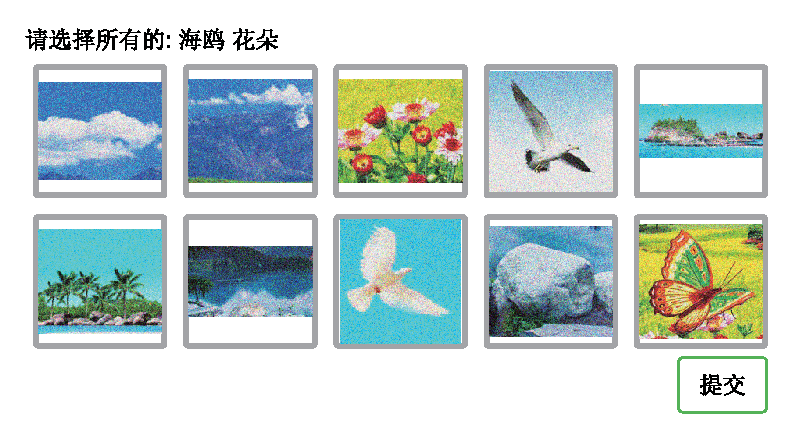
\includegraphics{pic/captcha-demo.eps}
\caption{一个自增长的图片验证码例子}\label{fig:captcha-demo}
\end{figure}

事实上在实际实现中,我们在提供给用户的\emph{主体}中增加一些噪声。添加的噪声位置可能是图片的中心也有可能是图片的边缘。我们同样也做一些颜色调整来防止机器人分类器简单的将噪声移除。这样的而随机噪声策略确保了每一张图片有不同的噪声等级。通这种方式能很好的提高系统鲁棒性。

\subsection{用户研究}\label{ux7528ux6237ux7814ux7a76}

用户友好性也是验证码系统设计需要考量的标准之一,我们结合reCAPTCHA和Asirra进行用户研究。Assira和reCAPTCHA在的web服务被大量使用,很容易被我们的研究集成进来。我们随机抽取100个男性和50个女性远程参加这个研究项目,其中大部分为在校生。在测试之前,我们给受试者一张画报,来告诉他们怎么通过测试,而我们则记录受试者完成每个\emph{问题}的时间和回答\emph{问题}的正确率和总尝试次数。

用户研究通过网页的形式进行,具体内容如下:

\begin{itemize}
\tightlist
\item
  基本信息:包括受试者的基本信息:对验证码的熟悉程度,年龄,性别,学历
\item
  验证码描述:描述我们的系统,reCAPTCHA和Assira,让用户了解如何解答验证码\emph{问题}。
\item
  5个不同的我们的验证码
\item
  5个不同的reCAPTCHA问题
\item
  5个不同的Assira问题
\item
  评价:让受试者对我们的系统,reCAPTCHA和Assira娱乐性,易用性进行打分
\end{itemize}

\subsubsection{时间统计}\label{ux65f6ux95f4ux7edfux8ba1}

\begin{figure}[htbp]
\centering
\includegraphics{pic/pdf.eps}
\caption{时间分布图}\label{fig:time-distribute}
\end{figure}

图~\ref{fig:time-distribute}
是用户完成测试的时间分布图。可以看出大部分数据都是均匀的,只有很少的数据偏离了主体,成为离散点。因此可以用平均时间代表大部分用户的行为。

\begin{longtable}[]{@{}ccccc@{}}
\caption{\label{tbl:time}几种验证码系统用户单个\emph{问题}平均解决时间
}\tabularnewline
\toprule
& 我们的系统 & reCAPTCHA & 12306 验证码 & Asirra\tabularnewline
\midrule
\endfirsthead
\toprule
& 我们的系统 & reCAPTCHA & 12306 验证码 & Asirra\tabularnewline
\midrule
\endhead
平均用时(秒) & 10.61 & 9.98 & 10.45 & 16.05\tabularnewline
\bottomrule
\end{longtable}

如 表~\ref{tbl:time} ,我们可以发现,用户解决我们的的系统用时与 12306
验证码相思;同时这两个验证码系统都与reCAPTCHA系统相似。这说明了,合理设置的图片验证码能与文本验证码一样,能让用户快速的解决。而Asirra系统在这一方面则逊色很多,用户需要花费较长的时间来解决\emph{问题}。这其中可能的原因是猫和狗的照片混合在一起,让人类也较难辨认。而我们的系统,图片中不仅仅可能出现猫和狗,还可能出现其他的\emph{主体},故我们的系统在保证用户友好的同时,还可以提供更高的安全性。

\subsubsection{精确度统计}\label{ux7cbeux786eux5ea6ux7edfux8ba1}

在真实使用场景中,验证码系统需哟啊对人类有很高的尝试正确率(C.A.R)。所谓``尝试正确率''是指正确的尝试除以所有尝试次数。这意味这人类需要验证多少次才能通过测试。这个数值越接近\(1\),系统的可用性越高。

\begin{longtable}[]{@{}ccccc@{}}
\caption{\label{tbl:accuracy}几种验证码系统平均尝试正确率
}\tabularnewline
\toprule
& 我们的系统 & reCAPTCHA & 12306 验证码 & Asirra\tabularnewline
\midrule
\endfirsthead
\toprule
& 我们的系统 & reCAPTCHA & 12306 验证码 & Asirra\tabularnewline
\midrule
\endhead
平均尝试正确率 & 0.94 & 0.85 & 0.93 & 0.91\tabularnewline
\bottomrule
\end{longtable}

如
表~\ref{tbl:accuracy},我们可以看到三种图片验证码系统用户尝试准确率更高。这其中的原因可能是文本验证码系统用户需要用键盘输入,而图片验证码系统用户只需要点击即可完成。这也就从侧面验证了图片验证码系统相比与文本验证码系统,有着更好的可用性。其中我们的系统和
12306
验证码系统正确相仿,并拥有四中验证码系统中最高的精确度。这个数据表明,我们的系统有着很好的可用性。

\subsubsection{娱乐性和易用性}\label{ux5a31ux4e50ux6027ux548cux6613ux7528ux6027}

在对比四个系统之后,用户被问及比较我们的系统和Assira的娱乐性和轻松性。打分标准如下:

\begin{itemize}
\tightlist
\item
  1,如果用户认为Assira有更好的娱乐性或易用性
\item
  3,如果用户认为Assira和我们的系统有相等的娱乐性或是易用性
\item
  5,如果用户认为我们的系统有更好的娱乐性或易用性
\item
  2或4,如果用户倾向于Assira或是我们的系统
\end{itemize}

\begin{figure}[htbp]
\centering

\includegraphics{pic/cqu.eps}
\caption{娱乐性打分分布}\label{fig:entertainment}
\end{figure}

这一因素较为主观,但能较好的反应用户对我们验证码系统的态度。可以清楚的从
图~\ref{fig:entertainment}
中看到,娱乐性这一因素,用户大体上认为我们的系统和Assira一致。

\begin{figure}[htbp]
\centering

\includegraphics{pic/cqu.eps}
\caption{易用性打分分布}\label{fig:easy-used}
\end{figure}

而在易用性这一指标上,如 图~\ref{fig:easy-used}
用户认为我们的系统更加易用。这个结果不难理解:对于Assira系统来说,用户需要辨认狗和猫,而有些图片对于人来说也是比较难辨认的,因此会降低用户评价。

\subsubsection{自增长策略}\label{ux81eaux589eux957fux7b56ux7565-1}

我们的系统拥有自增长特性,所以自增长的图片是否准确,增长速度是否比较快也是衡量系统好坏的关键因素。

在我们的用户测试中,一共进行\(150*5=750\)次成功测试,而用户进行的总尝试为\(798\)次;

\section{存在问题和改进空间}\label{ux5b58ux5728ux95eeux9898ux548cux6539ux8fdbux7a7aux95f4}

在我们的实现中,使用一个爬虫来爬取网页上的图片,进而生成\emph{主体}。可是在实际的使用中,爬取的图片并不一定是我们所希望的,有些图片本身并不带有主体;甚至有些图片会让人感到反感;爬取的图片可能还涉及法律问题。这些问题在实际使用中,是亟待解决的。

对于这个问题,较为理想的解决方案是再增加一个神经网络,其用来筛选图片。然而这个神经网络的实现相当复杂,考虑因素也很多,需要感兴趣的学者继续研究完成。

自增长的验证系统可能还存在一个很小的问题,这个问题发生概率极低,并且很容易规避:\emph{主体}预分类标签错误,并且错误的标签正好和某个\emph{问题}中真正其验证作用的\emph{主体}名称冲突,继而可能系统自增长可能统计到错误的数据。而这一问题是不需要解决的,因为:

\begin{itemize}
\tightlist
\item
  发生概率极低,对系统自增长影响微乎其微
\item
  系统本身有一定的鲁棒性:几次错误的统计并不会引起系统自增长决策失误,综合多个答案可以很好的规避这个问题。
\end{itemize}

在我们的简单实现中,使用一个类似与12306的图片验证码系统\textsuperscript{{[}24{]}}。针对图片验证码形式,其实还有更好的方案,即SEMAGE\textsuperscript{{[}33{]}};它的设计思想是把图片语义关联加入图片验证码中,进而提高系统鲁棒性。我们的验证码增长策略可以不修改或是很小修改即可适应SEMAGE系统。

\section{总结}\label{ux603bux7ed3}

\begin{thebibliography}{99}

\end{thebibliography}

\hypertarget{refs}{}
\hypertarget{ref-baird2002human}{}
{[}1{]} BAIRD H S, POPAT K. Human interactive proofs and document image
analysis{[}G{]}//Document Analysis Systems V. Springer, 2002: 507--518.

\hypertarget{ref-chellapilla2005designing}{}
{[}2{]} CHELLAPILLA K, LARSON K, SIMARD P, 等. Designing human friendly
human interaction proofs (HIPs){[}C{]}//Proceedings of the SIGCHI
conference on Human factors in computing systems. ACM, 2005: 711--720.

\hypertarget{ref-rui2003excuse}{}
{[}3{]} RUI Y, LIU Z. Excuse me, but are you human?{[}C{]}//Proceedings
of the eleventh ACM international conference on Multimedia. ACM, 2003:
462--463.

\hypertarget{ref-von2003captcha}{}
{[}4{]} VON AHN L, BLUM M, HOPPER N J, 等. CAPTCHA: Using hard AI
problems for security{[}G{]}//Advances in Cryptology---EUROCRYPT 2003.
Springer, 2003: 294--311.

\hypertarget{ref-von2004telling}{}
{[}5{]} VON AHN L, BLUM M, LANGFORD J. Telling humans and computers
apart automatically{[}J{]}. Communications of the ACM, ACM, 2004, 47(2):
56--60.

\hypertarget{ref-mori2003recognizing}{}
{[}6{]} MORI G, MALIK J. Recognizing objects in adversarial clutter:
Breaking a visual CAPTCHA{[}C{]}//Computer Vision and Pattern
Recognition, 2003. Proceedings. 2003 IEEE Computer Society Conference
on. IEEE, 2003, 1: I--134.

\hypertarget{ref-yan2008low}{}
{[}7{]} YAN J, EL AHMAD A S. A Low-cost Attack on a Microsoft
CAPTCHA{[}C{]}//Proceedings of the 15th ACM conference on Computer and
communications security. ACM, 2008: 543--554.

\hypertarget{ref-simard2005using}{}
{[}8{]} SIMARD P. Using machine learning to break visual human
interaction proofs (hips{[}J{]}. Advances in neural information
processing systems, 2005, 17: 265--272.

\hypertarget{ref-elson2007asirra}{}
{[}9{]} ELSON J, DOUCEUR J R, HOWELL J, 等. Asirra: a CAPTCHA that
exploits interest-aligned manual image categorization.{[}C{]}//2007.

\hypertarget{ref-gossweiler2009s}{}
{[}10{]} GOSSWEILER R, KAMVAR M, BALUJA S. What's up CAPTCHA?: a CAPTCHA
based on image orientation{[}C{]}//Proceedings of the 18th international
conference on World wide web. ACM, 2009: 841--850.

\hypertarget{ref-chew2004image}{}
{[}11{]} CHEW M, TYGAR J D. Image recognition captchas{[}M{]}. Springer,
2004.

\hypertarget{ref-datta2005imagination}{}
{[}12{]} DATTA R, LI J, WANG J Z. IMAGINATION: a robust image-based
CAPTCHA generation system{[}C{]}//Proceedings of the 13th annual ACM
international conference on Multimedia. ACM, 2005: 331--334.

\hypertarget{ref-matthews2010scene}{}
{[}13{]} MATTHEWS P, MANTEL A, ZOU C C. Scene tagging: image-based
CAPTCHA using image composition and object
relationships{[}C{]}//Proceedings of the 5th ACM Symposium on
Information, Computer and Communications Security. ACM, 2010: 345--350.

\hypertarget{ref-zhu2010attacks}{}
{[}14{]} ZHU B B, YAN J, LI Q, 等. Attacks and design of image
recognition CAPTCHAs{[}C{]}//Proceedings of the 17th ACM conference on
Computer and communications security. ACM, 2010: 187--200.

\hypertarget{ref-chan2003using}{}
{[}15{]} CHAN T-Y. Using a test-to-speech synthesizer to generate a
reverse Turing test{[}C{]}//Tools with Artificial Intelligence, 2003.
Proceedings. 15th IEEE International Conference on. IEEE, 2003:
226--232.

\hypertarget{ref-bigham2009evaluating}{}
{[}16{]} BIGHAM J P, CAVENDER A C. Evaluating existing audio CAPTCHAs
and an interface optimized for non-visual use{[}C{]}//Proceedings of the
SIGCHI Conference on Human Factors in Computing Systems. ACM, 2009:
1829--1838.

\hypertarget{ref-gimpy}{}
{[}17{]} Gimpy 项目{[}J{]}.
\url{http://www.captcha.net/captchas/gimpy/}.

\hypertarget{ref-el2010robustness}{}
{[}18{]} EL AHMAD A S, YAN J, MARSHALL L. The robustness of a new
CAPTCHA{[}C{]}//Proceedings of the Third European Workshop on System
Security. ACM, 2010: 36--41.

\hypertarget{ref-yan2008usability}{}
{[}19{]} YAN J, EL AHMAD A S. Usability of CAPTCHAs or usability issues
in CAPTCHA design{[}C{]}//Proceedings of the 4th symposium on Usable
privacy and security. ACM, 2008: 44--52.

\hypertarget{ref-googlerecaptcha}{}
{[}20{]} Google reCAPTCHA 项目{[}J{]}.
\url{https://www.google.com/recaptcha/intro/index.html}.

\hypertarget{ref-bursztein2011failure}{}
{[}21{]} BURSZTEIN E, BEAUXIS R, PASKOV H, 等. The failure of
noise-based non-continuous audio captchas{[}C{]}//Security and Privacy
(SP), 2011 IEEE Symposium on. IEEE, 2011: 19--31.

\hypertarget{ref-esp-pix}{}
{[}22{]} Esp-pix{[}J{]}.
\url{http://server251.theory.cs.cmu.edu/cgi-bin/esp-pix/esp-pix}.

\hypertarget{ref-sq-pix}{}
{[}23{]} Sq-pix{[}J{]}.
\url{http://server251.theory.cs.cmu.edu/cgi-bin/sq-pix}.

\hypertarget{ref-captcha12306}{}
{[}24{]} 12306验证码{[}J{]}. \url{https://kyfw.12306.cn/otn/login/init}.

\hypertarget{ref-ux8bb8ux65b0ux5f812015ux56feux50cfux5206ux5272ux7684ux65b0ux7406ux8bbaux548cux65b0ux65b9ux6cd5}{}
{[}25{]} 许新征, 丁世飞, 史忠植, 等. 图像分割的新理论和新方法{[}J{]}.
2015.

\hypertarget{ref-ux6797ux5f00ux989c2005ux5f69ux8272ux56feux50cfux5206ux5272ux65b9ux6cd5ux7efcux8ff0}{}
{[}26{]} 林开颜, 吴军辉, 徐立鸿, 等. 彩色图像分割方法综述{[}J{]}.
中国图象图形学报, 2005, 10(1): 1--10.

\hypertarget{ref-ux4e01ux4eae2010ux56feux50cfux5206ux5272ux65b9ux6cd5ux53caux6027ux80fdux8bc4ux4ef7ux7efcux8ff0}{}
{[}27{]} 丁亮, 张永平, 张雪英. 图像分割方法及性能评价综述{[}J{]}. 软件,
2010, 31(12): 78--83.

\hypertarget{ref-Felzenszwalb2004}{}
{[}28{]} FELZENSZWALB P F, HUTTENLOCHER D P. Efficient graph-based image
segmentation{[}J{]}. International Journal of Computer Vision, 2004,
59(2): 167--181.

\hypertarget{ref-le2015deep}{}
{[}29{]} LE D Q T, TIWARI S N, MERIALDO B. Deep Learning Image
Recognition{[}J{]}. 2015.

\hypertarget{ref-simonyan2014very}{}
{[}30{]} SIMONYAN K, ZISSERMAN A. Very deep convolutional networks for
large-scale image recognition{[}J{]}. arXiv preprint arXiv:1409.1556,
2014.

\hypertarget{ref-ciresan2012multi}{}
{[}31{]} CIRESAN D, MEIER U, SCHMIDHUBER J. Multi-column deep neural
networks for image classification{[}C{]}//Computer Vision and Pattern
Recognition (CVPR), 2012 IEEE Conference on. IEEE, 2012: 3642--3649.

\hypertarget{ref-ux5d14ux9526ux6cf01995ux5c0fux6ce2ux5206ux6790ux5bfcux8bba}{}
{[}32{]} 崔锦泰, 程正兴. 小波分析导论{[}J{]}. 西安: 西安交通大学出版社,
1995.

\hypertarget{ref-vikram2011semage}{}
{[}33{]} VIKRAM S, FAN Y, GU G. SEMAGE: a new image-based two-factor
CAPTCHA{[}C{]}//Proceedings of the 27th Annual Computer Security
Applications Conference. ACM, 2011: 237--246.

%\include{chapters/summery}

%%%%%%%%%%%%%%%%%%%%%%%%%%%%%%%%%%%%%%%



%\include{chapters/appendix}  %%附录

\end{document}
